\documentclass[varwidth=false, border=2pt]{standalone}

\usepackage{pgfplots}
\usepackage{tikz}
\usepackage{xcolor}

\begin{document}
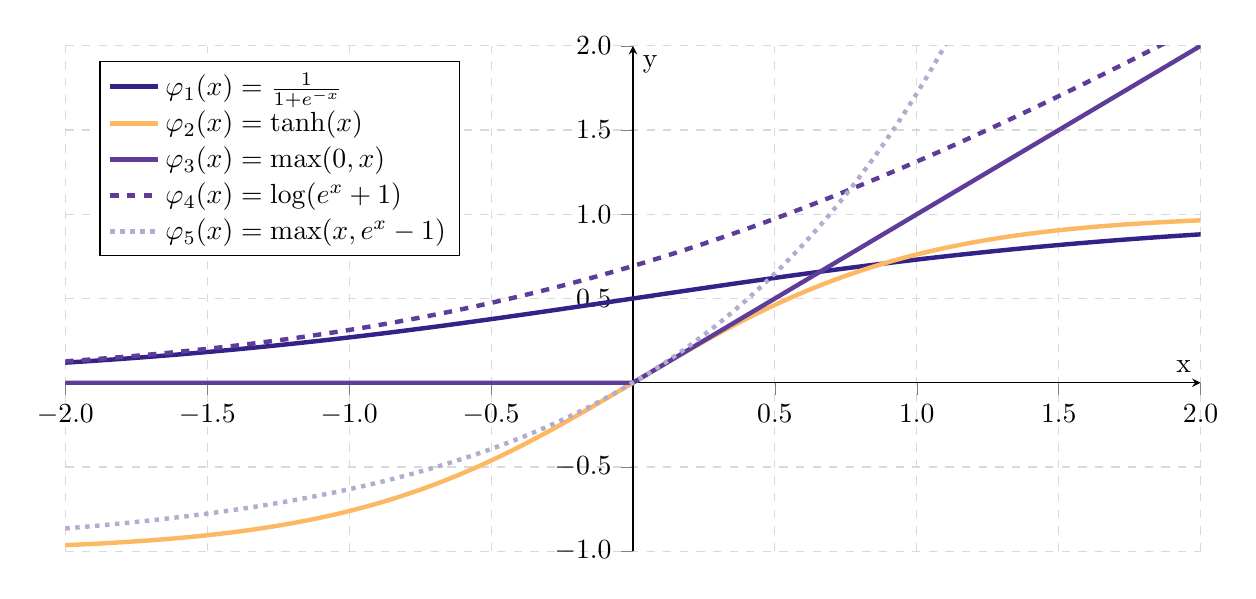
\begin{tikzpicture}
    \definecolor{color1}{HTML}{332288}
    \definecolor{color2}{HTML}{FDB863}
    \definecolor{color3}{HTML}{B2ABD2}
    \definecolor{color4}{HTML}{5E3C99}
    \begin{axis}[
        legend pos=north west,
        legend cell align={left},
        axis x line=middle,
        axis y line=middle,
        x tick label style={/pgf/number format/fixed,
                            /pgf/number format/fixed zerofill,
                            /pgf/number format/precision=1},
        y tick label style={/pgf/number format/fixed,
                            /pgf/number format/fixed zerofill,
                            /pgf/number format/precision=1},
        grid = major,
        width=16cm,
        height=8cm,
        grid style={dashed, gray!30},
        xmin=-2,     % start the diagram at this x-coordinate
        xmax= 2,    % end   the diagram at this x-coordinate
        ymin=-1,     % start the diagram at this y-coordinate
        ymax= 2,   % end   the diagram at this y-coordinate
        %axis background/.style={fill=white},
        xlabel=x,
        ylabel=y,
        tick align=outside,
        enlargelimits=false]
      % plot the stirling-formulae
      \addplot[domain=-2:2, color1, ultra thick,samples=500] {1/(1+exp(-x))};
      \addplot[domain=-2:2, color2, ultra thick,samples=500] {tanh(x)};
      \addplot[domain=-2:2, color4, ultra thick,samples=500] {max(0, x)};
      \addplot[domain=-2:2, color4, ultra thick,samples=500, dashed] {ln(exp(x) + 1)};
      \addplot[domain=-2:2, color3, ultra thick,samples=500, dotted] {max(x, exp(x) - 1)};
      \addlegendentry{$\varphi_1(x)=\frac{1}{1+e^{-x}}$}
      \addlegendentry{$\varphi_2(x)=\tanh(x)$}
      \addlegendentry{$\varphi_3(x)=\max(0, x)$}
      \addlegendentry{$\varphi_4(x)=\log(e^x + 1)$}
      \addlegendentry{$\varphi_5(x)=\max(x, e^x - 1)$}
    \end{axis}
\end{tikzpicture}
\end{document}
